\documentclass{article}

% ready for submission
\usepackage[final]{neurips_2023}
\usepackage{graphicx}
\usepackage[utf8]{inputenc} % allow utf-8 input
\usepackage[T1]{fontenc}    % use 8-bit T1 fonts
\usepackage{hyperref}       % hyperlinks
\usepackage{url}            % simple URL typesetting
\usepackage{booktabs}       % professional-quality tables
\usepackage{amsfonts}       % blackboard math symbols
\usepackage{nicefrac}       % compact symbols for 1/2, etc.
\usepackage{microtype}      % microtypography
\usepackage{xcolor}         % colors
% \usepackage{biblatex}       % Bibliographics
\bibliographystyle{abbrvnat}
\setcitestyle{authoryear,open={((},close={))}} %Citation-related commands


\title{Predicting Stocks with LSTM}

\author{%
  Elijah Moore \\
  Department of Electrical and Computer Engineering\\
  University of Alabama in Huntsville\\
  Huntsville, AL 35805 \\
  \texttt{elijah.moore@uah.edu} \\
}


\begin{document}


\maketitle


\begin{abstract}
  
\end{abstract}

\section{Introduction}

    Through the use of stock trading algorithms, large firms are able to take advantage of market corrections
    to turn a profit. The stock market/valuation of financial assets could be considered something of a stochastic system.
   
    This project uses some of the vast amounts of data available on finances to
    predict future trends in the stock market via a Long Short Term Model (LSTM).

\section{Literature Review}

    Predicting stocks is highly sought after for the purpose of trading, such that investors can maximize investment gains,
    and avoid devastating financial losses. As such, there are many articles published about methods of stock trading.

    Of these, Jakob Aungiers's work with LSTMs was notable for this work, with his framework used for LSTMs.
    Jakob used his famework for developing a prediction of the S\&P500, which was very good at predicting general trends.
    The key aspect of his work was creating a highly reconfigurable LSTM Framework. While not polished, the work enables rapid 
    changing of architecture of a model via a config.json file which allows the definition of new layers of the 
    neural network (NN), train test splits, epochs, dropout rate, batch sizes, loss functions, and Optimizers, 
    as well as the type of neurons in each layer without having to modify the python code.

\section{Design of Experiment}
    Yfinance's ticker module is used to access trading data on stocks.
    This yfinance submodule allows access to a larger number of input parameters than merely the price of the stock at a given moment.
    It also includes data about trades that are being made by `insiders' of a company, which would be useful for future iterations of this project.

    Additionally Keras was used for the LSTM Model

    The Apple (AAPL) stock and Ford (F) is evaluated based off of daily closing price over the last three years.

    The intent is to use a LSTM to predict the next days stock value, and trends in the stock's movement.

    The methods used here were very similar to Jakob Aungiers work with LSTMs in which the S\&P500 was predicted \cite[S\&P500]{web:lstm}.

    Using Jakob's framwork enabled rapid change and prototyping of different model types with reduced concern for syntactical
    issues \cite[framework]{web:lstmFramework}.

\section{Results}
    The first architecture used to predict the market used one layer with 100 neurons with a dense linear activation function.
    Additionally, it was configured to use a sequence of 50 data points. It converged after only 10 epochs, and had a final loss 
    value of 0.0112. The MSE Loss function was used.

    \begin{figure}
    \centering
    \fbox{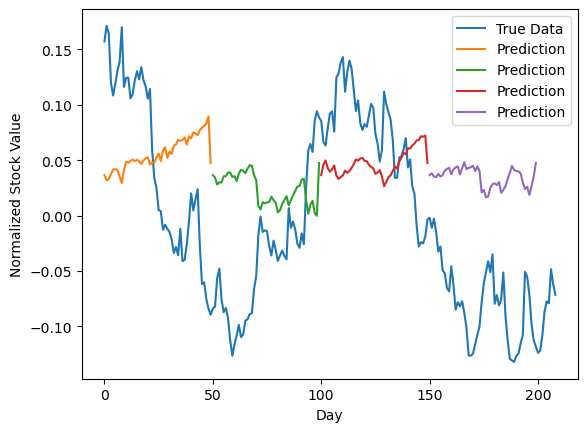
\includegraphics[width=0.5\columnwidth]{images/100by1plt.png}}
    \caption{Real stock data with prediction overlayed for the single layer 100 neuron LSTM.}
    \end{figure}

    Notably, as shown in Figure 1, the predicted values were similarly shaped to the stock, but still very different in location.
    In an effort to improve the model, the architectural file was changed to use 3 layers of 100 neurons, and also 
    introduce a dropout of 0.2 on the input and output layers.

    This model converged after 13 epochs to a final loss value of 0.0013, which is significantly better than the
    previous architecture. Despite this, the predicted stock is much smoother than the real data which would be fine
    if it predicted general trends, however as shown in Figure 2, the plot suggests it always predicts that the valued stock will decrease.

    \begin{figure}
        \centering
        \fbox{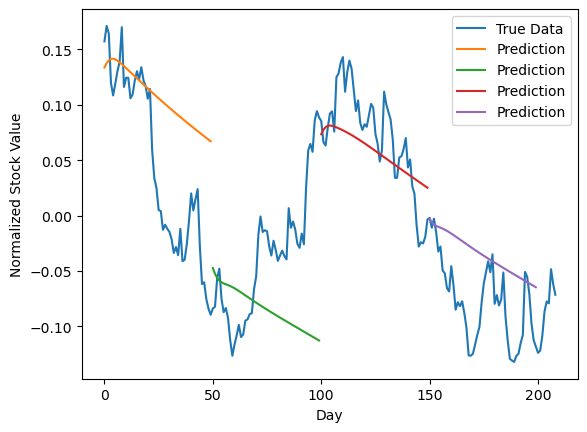
\includegraphics[width=0.5\columnwidth]{images/100by3withdropout.png}}
        \caption{Real stock data with prediction overlayed for the three layer 300 neuron LSTM on Apple.}
    \end{figure}

    To review this, the stock analyzed was changed from AAPL to Ford (F), while keeping all fo the same previous architectural
    choices. It once again converged after 13 epochs, but converged to a loss value of 0.0031. However the results appeared to 
    be much better when viewing predictions. In Figure 3, it is quite clear that the resulting predictions were 
    able to successfully predict a rise and a fall on the same stock. 

    

    \begin{figure}
        \centering
        \fbox{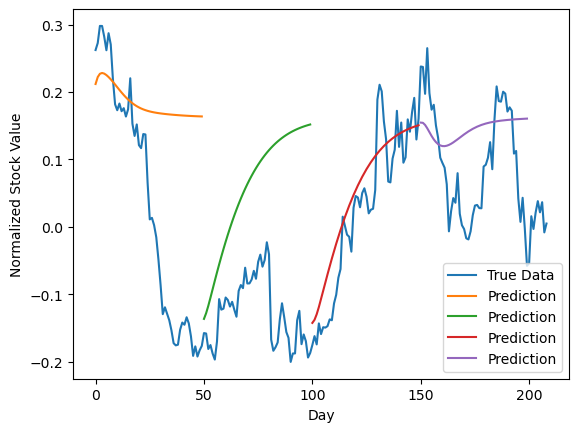
\includegraphics[width=0.5\columnwidth]{images/100by3withdropoutFord.png}}
        \caption{Real stock data with prediction overlayed for the three layer 300 neuron LSTM on Ford.}
    \end{figure}

\section{Conclusion}
    Despite this success, the trained model is likely overfit for the Ford stock, and additional research may be required to understand
    how to train an LSTM or other RNN on multiple datasets to prevent this. Additionally, the prediction of the Ford stock was
    very successful, while the prediction of the Apple stock was not particularly successful, perhaps this is due to more
    stochastic trends in the AAPL stock versus the F stock. 
    
    Overall, the complexity of the model and the inclusion of dropout greatly increased the 
    quality of this model. 

\begin{ack}

    No outside funding was recieved for this.


\end{ack}


% \section*{References}

% https://web.archive.org/web/20231117195704/https://altumintelligence.com/articles/a/Time-Series-Prediction-Using-LSTM-Deep-Neural-Networks

% https://www.jakob-aungiers.com/articles/a/LSTM-Neural-Network-for-Time-Series-Prediction

{
\small
    \nocite{*}
    \bibliography{ref}
}

%%%%%%%%%%%%%%%%%%%%%%%%%%%%%%%%%%%%%%%%%%%%%%%%%%%%%%%%%%%%


\end{document}